% Options for packages loaded elsewhere
\PassOptionsToPackage{unicode}{hyperref}
\PassOptionsToPackage{hyphens}{url}
%
\documentclass[
]{article}
\usepackage{lmodern}
\usepackage{amssymb,amsmath}
\usepackage{ifxetex,ifluatex}
\ifnum 0\ifxetex 1\fi\ifluatex 1\fi=0 % if pdftex
  \usepackage[T1]{fontenc}
  \usepackage[utf8]{inputenc}
  \usepackage{textcomp} % provide euro and other symbols
\else % if luatex or xetex
  \usepackage{unicode-math}
  \defaultfontfeatures{Scale=MatchLowercase}
  \defaultfontfeatures[\rmfamily]{Ligatures=TeX,Scale=1}
\fi
% Use upquote if available, for straight quotes in verbatim environments
\IfFileExists{upquote.sty}{\usepackage{upquote}}{}
\IfFileExists{microtype.sty}{% use microtype if available
  \usepackage[]{microtype}
  \UseMicrotypeSet[protrusion]{basicmath} % disable protrusion for tt fonts
}{}
\makeatletter
\@ifundefined{KOMAClassName}{% if non-KOMA class
  \IfFileExists{parskip.sty}{%
    \usepackage{parskip}
  }{% else
    \setlength{\parindent}{0pt}
    \setlength{\parskip}{6pt plus 2pt minus 1pt}}
}{% if KOMA class
  \KOMAoptions{parskip=half}}
\makeatother
\usepackage{xcolor}
\IfFileExists{xurl.sty}{\usepackage{xurl}}{} % add URL line breaks if available
\IfFileExists{bookmark.sty}{\usepackage{bookmark}}{\usepackage{hyperref}}
\hypersetup{
  pdftitle={Lab3},
  pdfauthor={Irimie Fabio},
  hidelinks,
  pdfcreator={LaTeX via pandoc}}
\urlstyle{same} % disable monospaced font for URLs
\usepackage[margin=1in]{geometry}
\usepackage{color}
\usepackage{fancyvrb}
\newcommand{\VerbBar}{|}
\newcommand{\VERB}{\Verb[commandchars=\\\{\}]}
\DefineVerbatimEnvironment{Highlighting}{Verbatim}{commandchars=\\\{\}}
% Add ',fontsize=\small' for more characters per line
\usepackage{framed}
\definecolor{shadecolor}{RGB}{248,248,248}
\newenvironment{Shaded}{\begin{snugshade}}{\end{snugshade}}
\newcommand{\AlertTok}[1]{\textcolor[rgb]{0.94,0.16,0.16}{#1}}
\newcommand{\AnnotationTok}[1]{\textcolor[rgb]{0.56,0.35,0.01}{\textbf{\textit{#1}}}}
\newcommand{\AttributeTok}[1]{\textcolor[rgb]{0.77,0.63,0.00}{#1}}
\newcommand{\BaseNTok}[1]{\textcolor[rgb]{0.00,0.00,0.81}{#1}}
\newcommand{\BuiltInTok}[1]{#1}
\newcommand{\CharTok}[1]{\textcolor[rgb]{0.31,0.60,0.02}{#1}}
\newcommand{\CommentTok}[1]{\textcolor[rgb]{0.56,0.35,0.01}{\textit{#1}}}
\newcommand{\CommentVarTok}[1]{\textcolor[rgb]{0.56,0.35,0.01}{\textbf{\textit{#1}}}}
\newcommand{\ConstantTok}[1]{\textcolor[rgb]{0.00,0.00,0.00}{#1}}
\newcommand{\ControlFlowTok}[1]{\textcolor[rgb]{0.13,0.29,0.53}{\textbf{#1}}}
\newcommand{\DataTypeTok}[1]{\textcolor[rgb]{0.13,0.29,0.53}{#1}}
\newcommand{\DecValTok}[1]{\textcolor[rgb]{0.00,0.00,0.81}{#1}}
\newcommand{\DocumentationTok}[1]{\textcolor[rgb]{0.56,0.35,0.01}{\textbf{\textit{#1}}}}
\newcommand{\ErrorTok}[1]{\textcolor[rgb]{0.64,0.00,0.00}{\textbf{#1}}}
\newcommand{\ExtensionTok}[1]{#1}
\newcommand{\FloatTok}[1]{\textcolor[rgb]{0.00,0.00,0.81}{#1}}
\newcommand{\FunctionTok}[1]{\textcolor[rgb]{0.00,0.00,0.00}{#1}}
\newcommand{\ImportTok}[1]{#1}
\newcommand{\InformationTok}[1]{\textcolor[rgb]{0.56,0.35,0.01}{\textbf{\textit{#1}}}}
\newcommand{\KeywordTok}[1]{\textcolor[rgb]{0.13,0.29,0.53}{\textbf{#1}}}
\newcommand{\NormalTok}[1]{#1}
\newcommand{\OperatorTok}[1]{\textcolor[rgb]{0.81,0.36,0.00}{\textbf{#1}}}
\newcommand{\OtherTok}[1]{\textcolor[rgb]{0.56,0.35,0.01}{#1}}
\newcommand{\PreprocessorTok}[1]{\textcolor[rgb]{0.56,0.35,0.01}{\textit{#1}}}
\newcommand{\RegionMarkerTok}[1]{#1}
\newcommand{\SpecialCharTok}[1]{\textcolor[rgb]{0.00,0.00,0.00}{#1}}
\newcommand{\SpecialStringTok}[1]{\textcolor[rgb]{0.31,0.60,0.02}{#1}}
\newcommand{\StringTok}[1]{\textcolor[rgb]{0.31,0.60,0.02}{#1}}
\newcommand{\VariableTok}[1]{\textcolor[rgb]{0.00,0.00,0.00}{#1}}
\newcommand{\VerbatimStringTok}[1]{\textcolor[rgb]{0.31,0.60,0.02}{#1}}
\newcommand{\WarningTok}[1]{\textcolor[rgb]{0.56,0.35,0.01}{\textbf{\textit{#1}}}}
\usepackage{graphicx}
\makeatletter
\def\maxwidth{\ifdim\Gin@nat@width>\linewidth\linewidth\else\Gin@nat@width\fi}
\def\maxheight{\ifdim\Gin@nat@height>\textheight\textheight\else\Gin@nat@height\fi}
\makeatother
% Scale images if necessary, so that they will not overflow the page
% margins by default, and it is still possible to overwrite the defaults
% using explicit options in \includegraphics[width, height, ...]{}
\setkeys{Gin}{width=\maxwidth,height=\maxheight,keepaspectratio}
% Set default figure placement to htbp
\makeatletter
\def\fps@figure{htbp}
\makeatother
\setlength{\emergencystretch}{3em} % prevent overfull lines
\providecommand{\tightlist}{%
  \setlength{\itemsep}{0pt}\setlength{\parskip}{0pt}}
\setcounter{secnumdepth}{-\maxdimen} % remove section numbering

\title{Lab3}
\usepackage{etoolbox}
\makeatletter
\providecommand{\subtitle}[1]{% add subtitle to \maketitle
  \apptocmd{\@title}{\par {\large #1 \par}}{}{}
}
\makeatother
\subtitle{Exercises}
\author{Irimie Fabio}
\date{}

\begin{document}
\maketitle

{
\setcounter{tocdepth}{2}
\tableofcontents
}
\hypertarget{exercise-1}{%
\section{Exercise 1}\label{exercise-1}}

\hypertarget{a}{%
\subsection{A}\label{a}}

Create the Lab3 project. Use the same structure used for Lab1 and Lab2:
scripts, plots and data directories.

\hypertarget{b}{%
\subsection{B}\label{b}}

Write a function to calculate the sum of integer numbers from 1 to n

\begin{Shaded}
\begin{Highlighting}[]
\NormalTok{sum\_integer \textless{}{-}}\StringTok{ }\ControlFlowTok{function}\NormalTok{(n) \{}
\NormalTok{  sum \textless{}{-}}\StringTok{ }\DecValTok{0}
  \ControlFlowTok{for}\NormalTok{ (i }\ControlFlowTok{in} \DecValTok{1}\OperatorTok{:}\NormalTok{n) \{}
\NormalTok{    sum \textless{}{-}}\StringTok{ }\NormalTok{sum }\OperatorTok{+}\StringTok{ }\NormalTok{i}
\NormalTok{  \}}
  \KeywordTok{return}\NormalTok{(sum)}
\NormalTok{\}}

\KeywordTok{cat}\NormalTok{(}\StringTok{"The sum of the first 10 integers is: "}\NormalTok{, }\KeywordTok{sum\_integer}\NormalTok{(}\DecValTok{10}\NormalTok{), }\StringTok{"}\CharTok{\textbackslash{}n}\StringTok{"}\NormalTok{)}
\end{Highlighting}
\end{Shaded}

\begin{verbatim}
## The sum of the first 10 integers is:  55
\end{verbatim}

\hypertarget{c}{%
\subsection{C}\label{c}}

Write a function to calculate the product of integers from 1 to n, also
known as n!

\begin{Shaded}
\begin{Highlighting}[]
\NormalTok{prod\_integer \textless{}{-}}\StringTok{ }\ControlFlowTok{function}\NormalTok{(n) \{}
\NormalTok{  val \textless{}{-}}\StringTok{ }\NormalTok{n}
  \ControlFlowTok{for}\NormalTok{ (i }\ControlFlowTok{in}\NormalTok{ (n }\OperatorTok{{-}}\StringTok{ }\DecValTok{1}\NormalTok{)}\OperatorTok{:}\DecValTok{1}\NormalTok{) \{}
\NormalTok{    val \textless{}{-}}\StringTok{ }\NormalTok{val }\OperatorTok{*}\StringTok{ }\NormalTok{i}
\NormalTok{  \}}
  \KeywordTok{return}\NormalTok{(val)}
\NormalTok{\}}

\KeywordTok{cat}\NormalTok{(}\StringTok{"The factorial of 5 is: "}\NormalTok{, }\KeywordTok{prod\_integer}\NormalTok{(}\DecValTok{5}\NormalTok{), }\StringTok{"}\CharTok{\textbackslash{}n}\StringTok{"}\NormalTok{)}
\end{Highlighting}
\end{Shaded}

\begin{verbatim}
## The factorial of 5 is:  120
\end{verbatim}

\hypertarget{d}{%
\subsection{D}\label{d}}

Try C. but do it recursively (hint: call the function itself inside the
loop, remember to return 1 when n is equal to 0)

\begin{Shaded}
\begin{Highlighting}[]
\NormalTok{factorial \textless{}{-}}\StringTok{ }\ControlFlowTok{function}\NormalTok{(n) \{}
  \ControlFlowTok{if}\NormalTok{ (n }\OperatorTok{==}\StringTok{ }\DecValTok{0}\NormalTok{) \{}
    \KeywordTok{return}\NormalTok{(}\DecValTok{1}\NormalTok{)}
\NormalTok{  \} }\ControlFlowTok{else}\NormalTok{ \{}
\NormalTok{    val \textless{}{-}}\StringTok{ }\NormalTok{n }\OperatorTok{*}\StringTok{ }\KeywordTok{factorial}\NormalTok{(n }\OperatorTok{{-}}\StringTok{ }\DecValTok{1}\NormalTok{)}
\NormalTok{  \}}

  \KeywordTok{return}\NormalTok{(val)}
\NormalTok{\}}

\KeywordTok{cat}\NormalTok{(}\StringTok{"The factorial of 5 is: "}\NormalTok{, }\KeywordTok{factorial}\NormalTok{(}\DecValTok{5}\NormalTok{), }\StringTok{"}\CharTok{\textbackslash{}n}\StringTok{"}\NormalTok{)}
\end{Highlighting}
\end{Shaded}

\begin{verbatim}
## The factorial of 5 is:  120
\end{verbatim}

\hypertarget{exercise-2}{%
\section{Exercise 2}\label{exercise-2}}

\hypertarget{a-1}{%
\subsection{A}\label{a-1}}

Simulate the tossing of a fair dice and verify through the definition
that the event \(E = \{ 2,3 \}\) has probability \(\frac{1}{3}\).
\(S = \{ 1,2,3,4,5,6 \}\); \(E = \{ 2,3 \}\); \(P(E) = \frac{1}{3}\)

(hint: generate a sequence of integer random numbers between 1 and 6
using the sample() function)

\begin{Shaded}
\begin{Highlighting}[]
\KeywordTok{library}\NormalTok{(ggplot2)}

\NormalTok{n \textless{}{-}}\StringTok{ }\DecValTok{100000} \CommentTok{\# Number of experiments}
\NormalTok{e \textless{}{-}}\StringTok{ }\KeywordTok{c}\NormalTok{(}\DecValTok{2}\NormalTok{, }\DecValTok{3}\NormalTok{) }\CommentTok{\# Event of interest}

\CommentTok{\# Outcomes of interest}
\KeywordTok{set.seed}\NormalTok{(}\DecValTok{123}\NormalTok{)}
\NormalTok{res \textless{}{-}}\StringTok{ }\KeywordTok{sample}\NormalTok{(}\DataTypeTok{x =} \KeywordTok{c}\NormalTok{(}\DecValTok{1}\OperatorTok{:}\DecValTok{6}\NormalTok{), }\DataTypeTok{size =}\NormalTok{ n, }\DataTypeTok{replace =} \OtherTok{TRUE}\NormalTok{)}

\CommentTok{\# Outcomes of E (1 when in E, 0 otherwise)}
\NormalTok{ne \textless{}{-}}\StringTok{ }\KeywordTok{ifelse}\NormalTok{(res }\OperatorTok{\%in\%}\StringTok{ }\NormalTok{e, }\DecValTok{1}\NormalTok{, }\DecValTok{0}\NormalTok{)}
\end{Highlighting}
\end{Shaded}

\hypertarget{b-1}{%
\subsection{B}\label{b-1}}

Plot the first 40 outcomes of the experiment.

\begin{Shaded}
\begin{Highlighting}[]
\KeywordTok{ggplot}\NormalTok{(}
  \DataTypeTok{data =} \KeywordTok{data.frame}\NormalTok{(}\DataTypeTok{x =} \DecValTok{1}\OperatorTok{:}\DecValTok{40}\NormalTok{, }\DataTypeTok{y =}\NormalTok{ res[}\DecValTok{1}\OperatorTok{:}\DecValTok{40}\NormalTok{]),}
  \KeywordTok{aes}\NormalTok{(}
    \DataTypeTok{x =}\NormalTok{ x,}
    \DataTypeTok{y =}\NormalTok{ y,}
    \DataTypeTok{color =} \KeywordTok{factor}\NormalTok{(res[}\DecValTok{1}\OperatorTok{:}\DecValTok{40}\NormalTok{])}
\NormalTok{  )}
\NormalTok{) }\OperatorTok{+}
\StringTok{  }\KeywordTok{geom\_point}\NormalTok{() }\OperatorTok{+}
\StringTok{  }\KeywordTok{scale\_color\_manual}\NormalTok{(}\DataTypeTok{values =} \KeywordTok{rainbow}\NormalTok{(}\DecValTok{6}\NormalTok{)) }\OperatorTok{+}
\StringTok{  }\KeywordTok{labs}\NormalTok{(}
    \DataTypeTok{title =} \StringTok{"First 40 outcomes of the dice"}\NormalTok{,}
    \DataTypeTok{x =} \StringTok{"Number of experiments"}\NormalTok{, }\DataTypeTok{y =} \StringTok{"Value"}
\NormalTok{  )}
\end{Highlighting}
\end{Shaded}

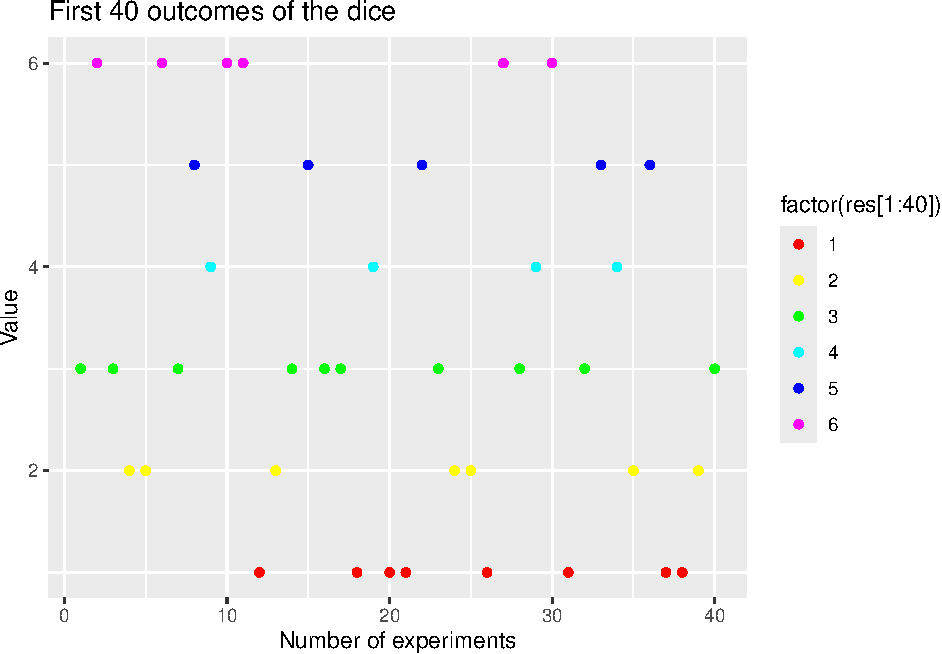
\includegraphics{es_files/figure-latex/unnamed-chunk-5-1.pdf}

\hypertarget{c-1}{%
\subsection{C}\label{c-1}}

Plot the convergence of \(P(E)\) at the value obtained from the
classical definition \(\frac{1}{3}\). (hint: the frequentist approach
says that, as the number of trials approaches infinity, the relative
frequency will converge exactly to the true probability)

\begin{Shaded}
\begin{Highlighting}[]
\CommentTok{\# Probability of E}
\NormalTok{pe \textless{}{-}}\StringTok{ }\KeywordTok{sum}\NormalTok{(ne) }\OperatorTok{/}\StringTok{ }\NormalTok{n}
\KeywordTok{cat}\NormalTok{(}\StringTok{"The probability of E is: "}\NormalTok{, pe, }\StringTok{"}\CharTok{\textbackslash{}n}\StringTok{"}\NormalTok{)}
\end{Highlighting}
\end{Shaded}

\begin{verbatim}
## The probability of E is:  0.33474
\end{verbatim}

\begin{Shaded}
\begin{Highlighting}[]
\NormalTok{cum\_pe \textless{}{-}}\StringTok{ }\KeywordTok{cumsum}\NormalTok{(ne) }\OperatorTok{/}\StringTok{ }\DecValTok{1}\OperatorTok{:}\NormalTok{n}

\NormalTok{df \textless{}{-}}\StringTok{ }\KeywordTok{data.frame}\NormalTok{(}\DataTypeTok{x =} \DecValTok{1}\OperatorTok{:}\NormalTok{n, }\DataTypeTok{y =}\NormalTok{ cum\_pe)}
\KeywordTok{ggplot}\NormalTok{(}\DataTypeTok{data =}\NormalTok{ df, }\KeywordTok{aes}\NormalTok{(}
  \DataTypeTok{x =}\NormalTok{ x, }\DataTypeTok{y =}\NormalTok{ y,}
\NormalTok{)) }\OperatorTok{+}
\StringTok{  }\KeywordTok{geom\_line}\NormalTok{() }\OperatorTok{+}
\StringTok{  }\KeywordTok{geom\_hline}\NormalTok{(}\DataTypeTok{yintercept =} \DecValTok{1} \OperatorTok{/}\StringTok{ }\DecValTok{3}\NormalTok{, }\DataTypeTok{col =} \StringTok{"red"}\NormalTok{) }\OperatorTok{+}
\StringTok{  }\KeywordTok{scale\_x\_continuous}\NormalTok{(}\DataTypeTok{trans =} \StringTok{"log10"}\NormalTok{) }\OperatorTok{+}
\StringTok{  }\KeywordTok{labs}\NormalTok{(}
    \DataTypeTok{title =} \StringTok{"Cumulative probability of E"}\NormalTok{,}
    \DataTypeTok{x =} \StringTok{"Number of experiments"}\NormalTok{, }\DataTypeTok{y =} \StringTok{"Cumulative probability"}
\NormalTok{  )}
\end{Highlighting}
\end{Shaded}

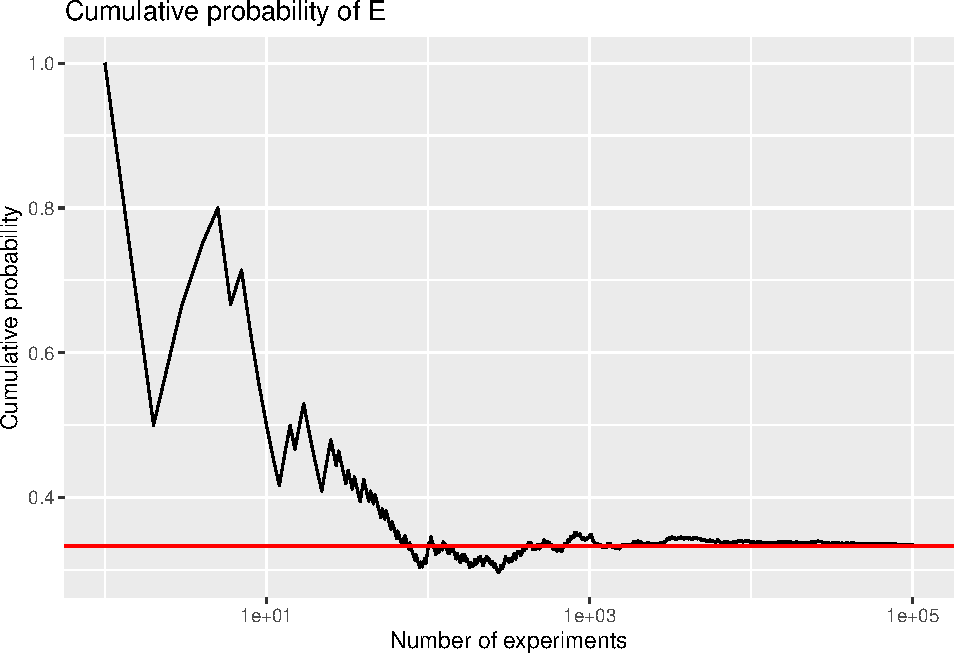
\includegraphics{es_files/figure-latex/unnamed-chunk-6-1.pdf}

\hypertarget{exercise-3}{%
\section{Exercise 3}\label{exercise-3}}

\hypertarget{a-2}{%
\subsection{A}\label{a-2}}

Simulate the tossing of a fair dice and consider the following events:
\(A=\{1,2\};\;B=\{2,3,6\};\;C=\{1,4,5\}\). (hint: compute
\(P(A),P(B),P(C)\)).

\begin{Shaded}
\begin{Highlighting}[]
\NormalTok{n \textless{}{-}}\StringTok{ }\DecValTok{100000} \CommentTok{\# Number of experiments}

\NormalTok{a \textless{}{-}}\StringTok{ }\KeywordTok{c}\NormalTok{(}\DecValTok{1}\NormalTok{, }\DecValTok{2}\NormalTok{) }\CommentTok{\# Event A}
\NormalTok{b \textless{}{-}}\StringTok{ }\KeywordTok{c}\NormalTok{(}\DecValTok{2}\NormalTok{, }\DecValTok{3}\NormalTok{, }\DecValTok{6}\NormalTok{) }\CommentTok{\# Event B}
\NormalTok{c \textless{}{-}}\StringTok{ }\KeywordTok{c}\NormalTok{(}\DecValTok{1}\NormalTok{, }\DecValTok{4}\NormalTok{, }\DecValTok{5}\NormalTok{) }\CommentTok{\# Event C}

\NormalTok{res \textless{}{-}}\StringTok{ }\KeywordTok{sample}\NormalTok{(}\DataTypeTok{x =} \KeywordTok{c}\NormalTok{(}\DecValTok{1}\OperatorTok{:}\DecValTok{6}\NormalTok{), }\DataTypeTok{size =}\NormalTok{ n, }\DataTypeTok{replace =} \OtherTok{TRUE}\NormalTok{)}

\NormalTok{pa \textless{}{-}}\StringTok{ }\KeywordTok{sum}\NormalTok{(res }\OperatorTok{\%in\%}\StringTok{ }\NormalTok{a) }\OperatorTok{/}\StringTok{ }\NormalTok{n}
\NormalTok{pa}
\CommentTok{\#\# [1] 0.33191}
\NormalTok{pb \textless{}{-}}\StringTok{ }\KeywordTok{sum}\NormalTok{(res }\OperatorTok{\%in\%}\StringTok{ }\NormalTok{b) }\OperatorTok{/}\StringTok{ }\NormalTok{n}
\NormalTok{pb}
\CommentTok{\#\# [1] 0.50041}
\NormalTok{pc \textless{}{-}}\StringTok{ }\KeywordTok{sum}\NormalTok{(res }\OperatorTok{\%in\%}\StringTok{ }\NormalTok{c) }\OperatorTok{/}\StringTok{ }\NormalTok{n}
\NormalTok{pc}
\CommentTok{\#\# [1] 0.49959}
\end{Highlighting}
\end{Shaded}

\hypertarget{b-2}{%
\subsection{B}\label{b-2}}

Verify that \(A\) and \(B\) are independent and that \(B\) and \(C\) are
dependent.

\begin{Shaded}
\begin{Highlighting}[]
\CommentTok{\# A and B}
\NormalTok{pab \textless{}{-}}\StringTok{ }\KeywordTok{sum}\NormalTok{(res }\OperatorTok{\%in\%}\StringTok{ }\NormalTok{a }\OperatorTok{\&}\StringTok{ }\NormalTok{res }\OperatorTok{\%in\%}\StringTok{ }\NormalTok{b) }\OperatorTok{/}\StringTok{ }\NormalTok{n}

\CommentTok{\# B and C}
\NormalTok{pbc \textless{}{-}}\StringTok{ }\KeywordTok{sum}\NormalTok{(res }\OperatorTok{\%in\%}\StringTok{ }\NormalTok{b }\OperatorTok{\&}\StringTok{ }\NormalTok{res }\OperatorTok{\%in\%}\StringTok{ }\NormalTok{c) }\OperatorTok{/}\StringTok{ }\NormalTok{n}

\KeywordTok{cat}\NormalTok{(}\StringTok{"A and B are independent: "}\NormalTok{, pab }\OperatorTok{==}\StringTok{ }\NormalTok{pa }\OperatorTok{*}\StringTok{ }\NormalTok{pb, }\StringTok{"}\CharTok{\textbackslash{}n}\StringTok{"}\NormalTok{)}
\end{Highlighting}
\end{Shaded}

\begin{verbatim}
## A and B are independent:  FALSE
\end{verbatim}

\begin{Shaded}
\begin{Highlighting}[]
\KeywordTok{cat}\NormalTok{(}\StringTok{"B and C are dependent: "}\NormalTok{, pbc }\OperatorTok{!=}\StringTok{ }\NormalTok{pb }\OperatorTok{*}\StringTok{ }\NormalTok{pc, }\StringTok{"}\CharTok{\textbackslash{}n}\StringTok{"}\NormalTok{)}
\end{Highlighting}
\end{Shaded}

\begin{verbatim}
## B and C are dependent:  TRUE
\end{verbatim}

\hypertarget{exercise-4}{%
\section{Exercise 4}\label{exercise-4}}

\hypertarget{a-3}{%
\subsection{A}\label{a-3}}

Generate a sequence of \(N=10000\) random numbers that simulate the
throwing of a dice.

\begin{Shaded}
\begin{Highlighting}[]
\NormalTok{n \textless{}{-}}\StringTok{ }\DecValTok{10000}
\KeywordTok{set.seed}\NormalTok{(}\DecValTok{123}\NormalTok{)}
\NormalTok{res \textless{}{-}}\StringTok{ }\KeywordTok{sample}\NormalTok{(}\DataTypeTok{x =} \KeywordTok{c}\NormalTok{(}\DecValTok{1}\OperatorTok{:}\DecValTok{6}\NormalTok{), }\DataTypeTok{size =}\NormalTok{ n, }\DataTypeTok{replace =} \OtherTok{TRUE}\NormalTok{)}
\end{Highlighting}
\end{Shaded}

\hypertarget{b-3}{%
\subsection{B}\label{b-3}}

Then simulate the throwing of a second dice.

\begin{Shaded}
\begin{Highlighting}[]
\NormalTok{res2 \textless{}{-}}\StringTok{ }\KeywordTok{sample}\NormalTok{(}\DataTypeTok{x =} \KeywordTok{c}\NormalTok{(}\DecValTok{1}\OperatorTok{:}\DecValTok{6}\NormalTok{), }\DataTypeTok{size =}\NormalTok{ n, }\DataTypeTok{replace =} \OtherTok{TRUE}\NormalTok{)}
\end{Highlighting}
\end{Shaded}

\hypertarget{c-2}{%
\subsection{C}\label{c-2}}

Plot the absolute and relative frequencies for A. and the relative
frequency for the sum of the two dice for point B. using the geom\_bar()
or geom\_col() functions.

\begin{Shaded}
\begin{Highlighting}[]
\NormalTok{df1 \textless{}{-}}\StringTok{ }\KeywordTok{data.frame}\NormalTok{(}\DataTypeTok{x =} \DecValTok{1}\OperatorTok{:}\DecValTok{6}\NormalTok{, }\DataTypeTok{y =} \KeywordTok{table}\NormalTok{(res) }\OperatorTok{/}\StringTok{ }\NormalTok{n)}
\NormalTok{df2 \textless{}{-}}\StringTok{ }\KeywordTok{data.frame}\NormalTok{(}\DataTypeTok{x =} \DecValTok{2}\OperatorTok{:}\DecValTok{12}\NormalTok{, }\DataTypeTok{y =} \KeywordTok{table}\NormalTok{(res }\OperatorTok{+}\StringTok{ }\NormalTok{res2) }\OperatorTok{/}\StringTok{ }\NormalTok{n)}

\KeywordTok{ggplot}\NormalTok{(}\DataTypeTok{data =}\NormalTok{ df1, }\KeywordTok{aes}\NormalTok{(}
  \DataTypeTok{x =} \KeywordTok{factor}\NormalTok{(x),}
  \DataTypeTok{y =}\NormalTok{ y.Freq}
\NormalTok{)) }\OperatorTok{+}
\StringTok{  }\KeywordTok{geom\_col}\NormalTok{() }\OperatorTok{+}
\StringTok{  }\KeywordTok{labs}\NormalTok{(}
    \DataTypeTok{title =} \StringTok{"Absolute frequency of the dice"}\NormalTok{,}
    \DataTypeTok{x =} \StringTok{"Value"}\NormalTok{, }\DataTypeTok{y =} \StringTok{"Absolute frequency"}
\NormalTok{  ) }\OperatorTok{+}
\StringTok{  }\KeywordTok{theme\_minimal}\NormalTok{()}
\end{Highlighting}
\end{Shaded}

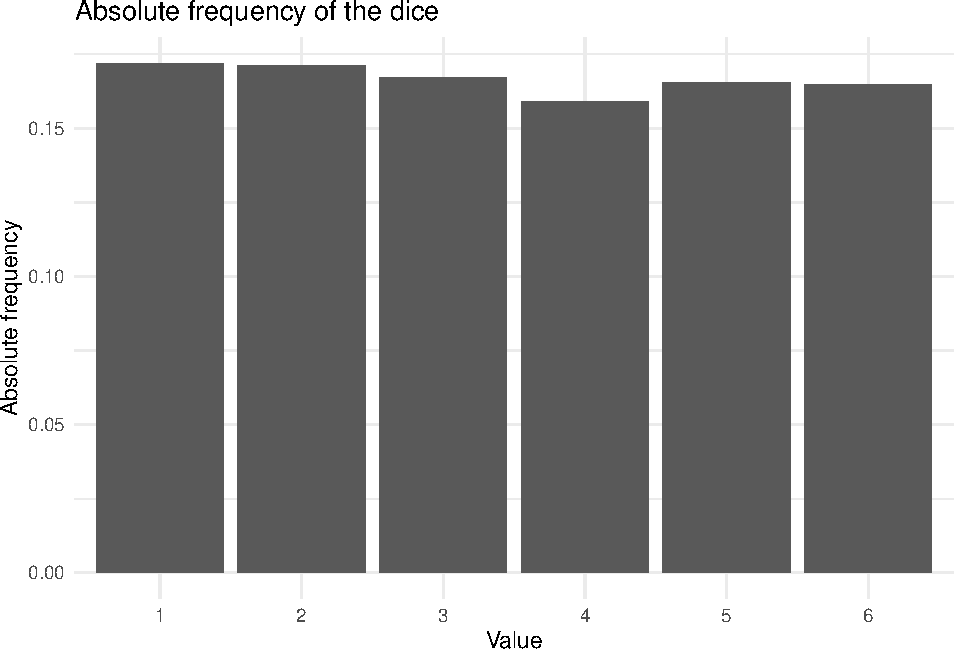
\includegraphics{es_files/figure-latex/unnamed-chunk-11-1.pdf}

\begin{Shaded}
\begin{Highlighting}[]
\KeywordTok{ggplot}\NormalTok{(}\DataTypeTok{data =}\NormalTok{ df2, }\KeywordTok{aes}\NormalTok{(}
  \DataTypeTok{x =} \KeywordTok{factor}\NormalTok{(x),}
  \DataTypeTok{y =}\NormalTok{ y.Freq}
\NormalTok{)) }\OperatorTok{+}
\StringTok{  }\KeywordTok{geom\_col}\NormalTok{() }\OperatorTok{+}
\StringTok{  }\KeywordTok{labs}\NormalTok{(}
    \DataTypeTok{title =} \StringTok{"Relative frequency of the sum of the dice"}\NormalTok{,}
    \DataTypeTok{x =} \StringTok{"Value"}\NormalTok{, }\DataTypeTok{y =} \StringTok{"Relative frequency"}
\NormalTok{  ) }\OperatorTok{+}
\StringTok{  }\KeywordTok{theme\_minimal}\NormalTok{()}
\end{Highlighting}
\end{Shaded}

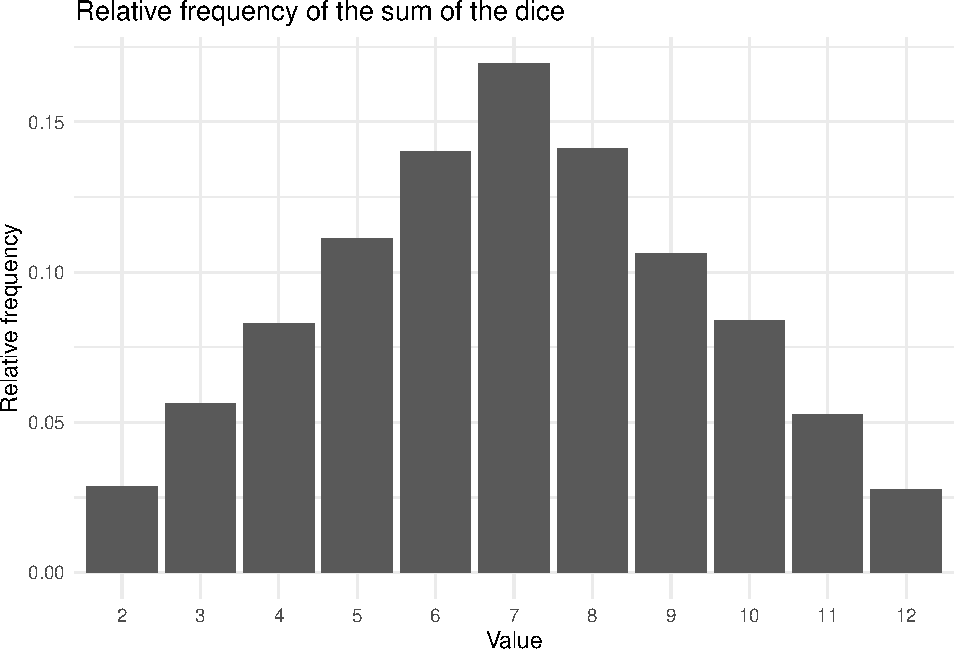
\includegraphics{es_files/figure-latex/unnamed-chunk-12-1.pdf}

\hypertarget{exercise-5}{%
\section{Exercise 5}\label{exercise-5}}

\hypertarget{a-4}{%
\subsection{A}\label{a-4}}

Four people are in a room. What is the probability that no two of them
celebrate their birthday on the same day of the year?

\begin{Shaded}
\begin{Highlighting}[]
\NormalTok{people \textless{}{-}}\StringTok{ }\DecValTok{4}
\NormalTok{days \textless{}{-}}\StringTok{ }\DecValTok{365}

\NormalTok{n\_bdays \textless{}{-}}\StringTok{ }\KeywordTok{choose}\NormalTok{(days, people) }\OperatorTok{*}\StringTok{ }\KeywordTok{factorial}\NormalTok{(people)}
\NormalTok{p\_bdays \textless{}{-}}\StringTok{ }\NormalTok{n\_bdays }\OperatorTok{/}\StringTok{ }\NormalTok{days}\OperatorTok{\^{}}\NormalTok{people}
\NormalTok{p\_bdays}
\end{Highlighting}
\end{Shaded}

\begin{verbatim}
## [1] 0.9836441
\end{verbatim}

\hypertarget{b-4}{%
\subsection{B}\label{b-4}}

\(n\) people are in a room. What is the probability that no two of them
celebrate their birthday on the same day of the year? Try this with
\(n\) from 1 to 100 and plot the probability for each value of \(n\).

\begin{Shaded}
\begin{Highlighting}[]
\NormalTok{n \textless{}{-}}\StringTok{ }\DecValTok{100}
\NormalTok{p\_bdays \textless{}{-}}\StringTok{ }\KeywordTok{rep}\NormalTok{(}\OtherTok{NA}\NormalTok{, n)}

\ControlFlowTok{for}\NormalTok{ (i }\ControlFlowTok{in} \DecValTok{1}\OperatorTok{:}\NormalTok{n) \{}
\NormalTok{  p\_bdays[i] \textless{}{-}}\StringTok{ }\KeywordTok{choose}\NormalTok{(days, i) }\OperatorTok{*}\StringTok{ }\KeywordTok{factorial}\NormalTok{(i) }\OperatorTok{/}\StringTok{ }\NormalTok{days}\OperatorTok{\^{}}\NormalTok{i}
\NormalTok{\}}

\NormalTok{df \textless{}{-}}\StringTok{ }\KeywordTok{data.frame}\NormalTok{(}\DataTypeTok{x =} \DecValTok{1}\OperatorTok{:}\NormalTok{n, }\DataTypeTok{y =}\NormalTok{ p\_bdays)}
\KeywordTok{ggplot}\NormalTok{(}\DataTypeTok{data =}\NormalTok{ df, }\KeywordTok{aes}\NormalTok{(}
  \DataTypeTok{x =}\NormalTok{ x, }\DataTypeTok{y =}\NormalTok{ y}
\NormalTok{)) }\OperatorTok{+}
\StringTok{  }\KeywordTok{geom\_line}\NormalTok{() }\OperatorTok{+}
\StringTok{  }\KeywordTok{labs}\NormalTok{(}
    \DataTypeTok{title =} \StringTok{"Probability of no two people having the same birthday"}\NormalTok{,}
    \DataTypeTok{x =} \StringTok{"Number of people"}\NormalTok{, }\DataTypeTok{y =} \StringTok{"Probability"}
\NormalTok{  ) }\OperatorTok{+}
\StringTok{  }\KeywordTok{theme\_minimal}\NormalTok{()}
\end{Highlighting}
\end{Shaded}

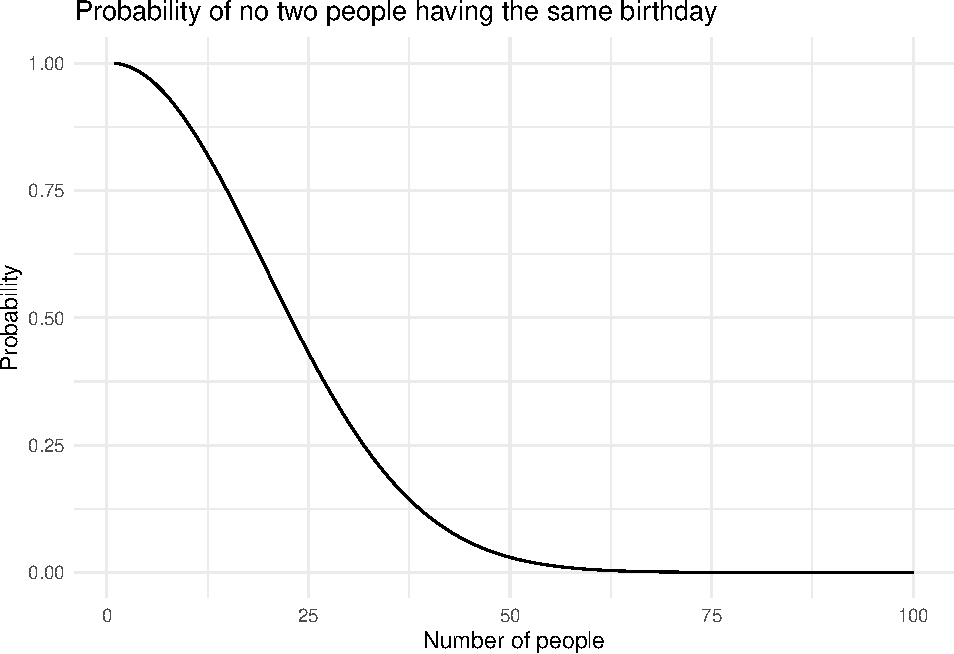
\includegraphics{es_files/figure-latex/unnamed-chunk-14-1.pdf}

\hypertarget{exercise-6}{%
\section{Exercise 6}\label{exercise-6}}

A laboratory blood test is 99\% effective in detecting a certain disease
when it is, in fact, present. However, the test also yields a ``false
positive'' (FP -- Type I error) result for 1\% of the healthy persons
tested. If 0.5\% of the population actually has the disease, what is the
probability a person has the disease given that his test result is
positive? (Hint: Use D as the event ``the tested person has the
disease'' and E as ``The result of the test is positive'').

\begin{Shaded}
\begin{Highlighting}[]
\NormalTok{p\_d \textless{}{-}}\StringTok{ }\FloatTok{0.005}
\NormalTok{p\_e\_d \textless{}{-}}\StringTok{ }\FloatTok{0.99}
\NormalTok{p\_e\_nd \textless{}{-}}\StringTok{ }\FloatTok{0.01}

\NormalTok{p\_d\_e \textless{}{-}}\StringTok{ }\NormalTok{p\_d }\OperatorTok{*}\StringTok{ }\NormalTok{p\_e\_d }\OperatorTok{/}\StringTok{ }\NormalTok{(p\_d }\OperatorTok{*}\StringTok{ }\NormalTok{p\_e\_d }\OperatorTok{+}\StringTok{ }\NormalTok{(}\DecValTok{1} \OperatorTok{{-}}\StringTok{ }\NormalTok{p\_d) }\OperatorTok{*}\StringTok{ }\NormalTok{p\_e\_nd)}
\NormalTok{p\_d\_e}
\end{Highlighting}
\end{Shaded}

\begin{verbatim}
## [1] 0.3322148
\end{verbatim}

\end{document}
